\documentclass[12pt,oneside,letterpaper]{article}
\usepackage{longtable}
\usepackage{float}
\usepackage{graphicx}
\usepackage{hyperref}

\newenvironment{packed_enumerate}{ %custom enumerate for single-spacing
\vspace{-7mm}
\begin{enumerate}
  \setlength{\itemsep}{0pt}
  \setlength{\parskip}{0pt}
  \setlength{\parsep}{0pt}
}{\end{enumerate}
\vspace{-8mm}}

\pagestyle{headings}
\oddsidemargin 0.25in \textwidth     6.25in \topmargin     0.4in
\textheight    8.5in

\begin{document}


\title{\bfseries Project Name: \\
Software Requirements Specification\\
version 4.0}

\author {
\large{Specific Atomics}\\
\emph{Computer Science Department}\\
\emph{California Polytechnic State University}\\
\emph{San Luis Obispo, CA USA}\\
}

\date{November 20, 2015}
\maketitle \thispagestyle{empty}


\pagebreak
\tableofcontents
\pagebreak

\addcontentsline{toc}{section}{Revision History}

\addcontentsline{toc}{section}{Credits}

\section*{Credits}
\begin{tabular}{|l|l|p{2.5in}|l|}
\hline
\textbf{Name} & \textbf{Date} & \textbf{Role} & \textbf{Version} \\
\hline
Alanna Buss & October 5, 2015 & Document Owner and Author & 3.5 \\
\hline
Dat Tran & October 5, 2015 & Author & 3.6 \\
\hline
Andrea Savage & October 5, 2015 & Author & 3.7 \\
\hline
Kevin Pham & October 5, 2015 & Author & 3.5 \\
\hline
Michael Lenz & October 5, 2015 & Author & 3.6 \\
\hline
Frank Poole & October 5, 2015 & Author & 4.2 \\
\hline
\end{tabular}

\addcontentsline{toc}{section}{Revision History}

\section*{Revision History}
\begin{tabular}{|l|l|p{2.5in}|l|}
\hline
\textbf{Name}&\textbf{Date}&\textbf{Reason for Changes}&\textbf{Version} \\
\hline
Alanna Buss & October 15, 2015 & Initial baseline approved by Customer & 1.0 \\
\hline
Alanna Buss&October 19, 2015&More use cases and use case name changes& 1.1 \\
\hline
Andrea Savage&October 21, 2015&Added Business Rules and Safety Requirements& 2.0 \\
\hline
Alanna Buss&October 25, 2015&Cleaned up receive use cases and did 6.3. Fixed use case numbering.& 3.0 \\
\hline
Alanna Buss&October 26, 2015&Added to the glossary & 3.2 \\
\hline
Andrea Savage &October 26, 2015&Added Correlation use cases and edited 6.2& 3.3 \\
\hline
Kevin Pham&October 26, 2015&Updated Use Case 3.19&3.3 \\
\hline
Frank Poole &October 26, 2015&Completed Simulate ADS-B Data Use Case&3.4 \\
\hline
Alanna Buss&October 27, 2015&Cleaned up section 6 & 3.5 \\
\hline
Michael Lenz&October 27, 2015&added Section 5.4 Communications Interfaces & 3.6 \\
\hline
Kevin Pham &October 27, 2015&completed sections 5.2 and 5.3 & 3.5 \\
\hline
Dat Tran &October 27, 2015&completed sections 4.8, 5.1, and 3.11 & 3.6 \\
\hline
Andrea Savage&October 28, 2015&Completed Use Cases 3.9 through 3.16, Completed 7C, Reformatted Section 5.4, and Revised SRS for continuity, grammar, and spelling& 3.7 \\
\hline
Frank Poole & November 20, 2015 & Edited Sections 1, 2, and 4 & 4.0 \\
\hline
Frank Poole & November 21, 2015 & Edited Section 4, 5, 6, and Appendices & 4.1 \\
\hline
Frank Poole & November 23, 2015 & Editing Section 5: UI Requirements & 4.2 \\
\hline
Alanna Buss&November 23, 2015& Fixing Send and Receive Use Cases&4.3\\
\hline
\end{tabular}

\newpage

\section{Introduction}
\subsection{Purpose}
This Software Requirements Specification describes the functional and nonfunctional software requirements for a research and development release of an unmanned aerial vehicle sense and avoid system. This document is intended to be used by the members of the project team who will implement and verify the correct functionality of the system. This document will also be used by our mentor, Dick Jay, and our direct supervisor, Dr. David Janzen.

\subsection{Document Conventions}
The following conventions are used in our document:
\begin{enumerate}
\item Links appear in a monospaced font.
\item GA-ASI the abbreviation for General Atomics Aeronautical Systems, Inc.
\item A byte refers to eight bits rather than the number of bits used to encode a single character of text on a central processing unit.
\item A float is understood as a floating point number of eight bytes.
\end{enumerate}

\subsection{Intended Audience and Reading Suggestions}

\subsubsection{Software Development Engineers}
Developers will primarily reference the functional and nonfunctional requirements. These requirements correspond to the features to be implemented. For the purposes of implementation, also referencing use cases may be helpful.\newline

\textit{Suggested Reading Sequence:}
\begin{enumerate}
\item Overall Description
\item System Features
\item Use Cases
\item External Interface Requirements
\item Other Nonfunctional Requirements
\end{enumerate}

\subsubsection{Software Quality Assurance Engineers}
Quality assurance personal will primarily reference the functional and nonfunctional requirements. The product features specified in this document will be tested by verifying the corresponding requirements using acceptance tests.\newline

\textit{Suggested Reading Sequence:}
\begin{enumerate}
\item Overall Description
\item System Features
\item External Interface Requirements
\item Other Nonfunctional Requirements
\end{enumerate}

\subsubsection{Software Product Owners and Customers}
Customers will observe and confirm that the specified features and requirements meet business needs and that all user needs are brought to attention. Additionally, they will serve a the primary product owner as they will prioritize features during implementation.\newline

\textit{Suggested Reading Sequence:}
\begin{enumerate}
\item Overall Description
\item System Features
\item Use Cases
\item External Interface Requirements
\item Other Nonfunctional Requirements
\end{enumerate}

\subsubsection{Management}
Management will remain informed of the team’s decisions and progress.\newline

\textit{Suggested Reading Sequence:}
\begin{enumerate}
\item Overall Description
\item System Features
\item External Interface Requirements
\item Other Nonfunctional Requirements
\end{enumerate}

\subsection{Project Scope}
This project will help further GA-ASI in their research and development of a sense and avoid system for unmanned aerial vehicles. Most modern aircraft currently have at least three different surveillance devices that each provide different types of data to its pilots. As the data can often conflict, the goal of this project is to design a system that will combine data from multiple devices: ADS-B, TCAS, and Radar in real time. The aggregated data will be presented on a visual display so that pilots or flight computers can avoid local objects. For additional information on the scope of this project, refer to the project Vision and Scope document listed as a reference.

\subsection{References}
\begin{enumerate}
\item\href{https://drive.google.com/file/d/0B-h6V6vvgmDkdDVxWmJkNXJSbFk/view}{Vision and Scope - Revision 1.0}break
\newline https://drive.google.com/file/d/0B-h6V6vvgmDkdDVxWmJkNXJSbFk/view
\item\href{https://drive.google.com/file/d/0B98KL9YVxK2nMXhEOVhqamFOanM/view}{Horizontal Prototype - Revision 1.0}
\newline https://drive.google.com/file/d/0B98KL9YVxK2nMXhEOVhqamFOanM/view
\item\href{https://drive.google.com/file/d/0B1Pa6phBjJfVUkNCNXVzZkRwWFU/view}{Development and Build Environment with Continuous Integration - Revision 1.0}
\newline https://drive.google.com/file/d/0B1Pa6phBjJfVUkNCNXVzZkRwWFU/view
\item\href{https://www.overleaf.com/3762327zdbpnb}{Glossary - Revision 1.0}
\newline https://www.overleaf.com/3762327zdbpnb
\end{enumerate}

\section{Overall Description}
\subsection{Product Perspective}
The sense and avoid engine is being designed as an add-on to the on board flight computer of unmanned aerial vehicles. The system will be connected to the TCAS, ADS-B, Radar, and ownship sensors already on board to gather data. In addition, it will output to either the autopilot or to a connected ground control station.\newline

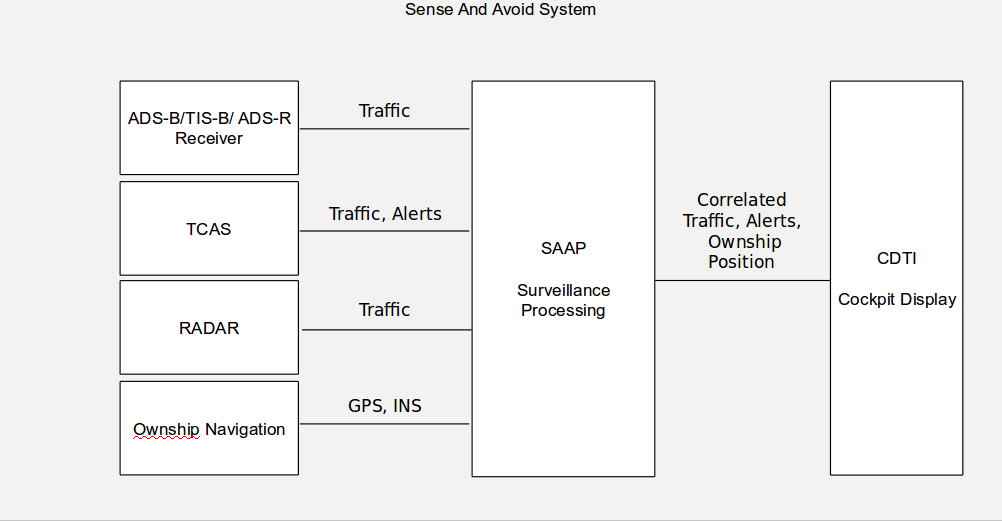
\includegraphics[scale=0.40]{system.png}\\

\subsection{Product Features}

\subsubsection{Surveillance Data Simulation}
\begin{enumerate}
\item Generate ADS-B data
\item Generate TCAS data
\item Generate Radar data
\item Generate ownship data
\end{enumerate}

\subsubsection{Surveillance Data Aggregation}
\begin{enumerate}
\item Read ADS-B data.
\item Read TCAS data.
\item Read Radar data.
\item Read ownship data.
\item Aggregate surveillance data from multiple sources.
\item Categorize detected objects by threat level.
\end{enumerate}

\subsubsection{Cockpit Display of Traffic Information}
\begin{enumerate}
\item Display aggregated surveillance data.
\end{enumerate}

\subsection{User Classes and Characteristics}
\begin{longtable}{|l|p{3.8in}|}
\hline
\textbf{User Class}&\textbf{Description}\\
\hline
Pilot & Monitors aircraft activity using the cockpit display of traffic information. The pilot will not be able to modify the display beyond interacting with easy to use buttons and switches.\\
\hline
Installer & Installs the sense and avoid system and performs initial configuration of the interface with the flight computer.\\
\hline
Engineer & Reviews flight logs and writes analyses and performance reviews. More specifically, engineers will be interested in reviewing the accuracy of the sense and avoid aggregation algorithm.\\
\hline
Administrator & Manages, delegates tasks, and assumes responsibility for running of the sense and avoid system.\\
\hline
\end{longtable}

\subsection{Operating Environment}
The Sense and Avoid Engine is ultimately intended to run on an embedded system contained within the electronics onboard an unmanned aerial vehicle. The software engine will run on a distribution of the Linux operating system. The application will have a dedicated processor and need not coexist with other software components.

\subsection{Design and Implementation Constraints}
\begin{enumerate}
\item The sense and avoid processing must be single threaded.
\item The sense and avoid processing occurs once per second.
\item Different surveillance devices have difference levels of data accuracy and rates of object detection.
\item ADS-B and TCAS will only report surveillance data for cooperative aircraft.
\item Radar reports data independently of intruder cooperativeness
\item The sense and avoid system is preferable written in C or C++ as these languages are industry standard.
\end{enumerate}

\subsection{User Documentation}
\begin{enumerate}
\item All executables will be delivered with a README file containing compilation instructions, execution instructions, and usage examples.
\item Any application programming interface documents for stand-alone components that may be reused in later research efforts.
\item Any test files used in the research and development of the sense and avoid processor.
\end{enumerate}

\subsection{Assumptions and Dependencies}
\subsubsection{Assumptions}
\begin{enumerate}
\item Research and development of an effective sense and avoid algorithm will require real and or simulated surveillance device data.
\end{enumerate}

\subsubsection{Dependencies}
\begin{enumerate}
\item Software Development activities will depend on the proper functioning of all technologies listed in the project Development and Build Environment with Continuous Integration document listed in the References section.
\item Design decisions may be limited by the dependence on the common data protocol shared by all research teams.
\item Any technologies used may later need to be used in the research and development of real unmanned aerial vehicles.
\end{enumerate}

\subsection{Business Rules}
\begin{itemize}
\item Br-1: If a plane is within 0.5 nautical miles and 50 feet of elevation of the ownship and the closest point of approach is less than 0.2 nautical miles and less than 5 seconds from the ownship, then the plane will crash.
\item Br-2: If a plane is within 2 nautical miles and 300 feet of elevation of the ownship and the closest point of approach is less than 0.5 nautical miles and less than 30 seconds from the ownship, then the plane will have a Resolution Advisory traffic type.
\item Br-3: If a plane is within 5 nautical miles and 500 feet of elevation of the ownship and the closest point of approach is less than 1 nautical mile and less than 60 seconds from the ownship, then the plane will have a Traffic Advisory traffic type.
\item Br-4: If a plane is within 10 nautical miles and 1000 feet of the ownship, then the plane will have a Proximate Traffic traffic type.
\end{itemize}

\section{Use Cases}

\subsection{\label{Sim Data}Use Case 1: Simulate Sensor Data}
\begin{longtable}{|r|p{3.8in}|}
\hline
Use Case ID:&1\\
\hline
Use Case Name:&Send Simulated Sensor Data\\
\hline
Created By:&Alanna Buss\\
\hline
Last Updated By:&Alanna Buss\\
\hline
Date Created:&November 24, 2015\\
\hline
Date Last Updated:&November 24, 2015\\
\hline
Actors:&The UAV Sense and Avoid Sensor Data Simulator; The UAV Sense and Avoid Sensor Data Aggregation Client\\
\hline
Description:&The simulator shall send ADS-B, TCAS, radar and ownship data to the Sense and Avoid Engine clients via a network connection.\\
\hline
Preconditions:&
\begin{packed_enumerate}
\item The simulator is on a network
\item The simulator and any clients are on the same network
\item The simulator has received the simulations flights from the Simulations Flight Generator.
\end{packed_enumerate}\\
\hline
Postconditions:&
\begin{packed_enumerate}
\item ADS-B data is formatted as described in Appendix B: ADS-B data
\item TCAS data is formatted as described in Appendix B: TCAS data
\item Radar data is formatted as described in Appendix B: Radar data
\item Ownship data is formatted as described in Appendix B: Ownship data
\end{packed_enumerate}\\
\hline
Normal Flow:&
\begin{packed_enumerate}
\item The simulator determines the next sensor data frame will be accurate
\item The simulator generates a data frame matching the type of sensor it is that is consistent with the data it received
\item The simulator determines it is the correct time to send the data
\item The simulator sends the data report over a network connection to all clients
\end{packed_enumerate}\\
\hline
Alternative Flows:&
\begin{packed_enumerate}
\item The simulator determines the next sensor data frame will not be accurate
\item The simulator generates a data frame matching the type of sensor it is that may not accurately reflect actual aircraft position
\item Continue from step 3 of the normal flow
\end{packed_enumerate}\\
\hline
Exceptions:&None\\
\hline
Includes:&None\\
\hline
Priority:&High\\
\hline
Frequency of Use:&1 Hz\\
\hline
Business Rules:&None\\
\hline
Special Requirements:&
\begin{packed_enumerate}
\item The simulator sends the data it creates asynchronously
\item The simulator generates accurate aircraft data for 99\% of the simulated ADS-B aircraft encounters and generates nominal data otherwise
\item The ADS-B sends up to 50 aircraft per second
\item The simulator generates accurate aircraft data for 85\% of the simulated TCAS aircraft encounters and generates nominal data otherwise
\item The TCAS sends up to 25 aircraft per second
\item The simulator generates accurate aircraft data for 90\% of the simulated Radar aircraft encounters and generates nominal data otherwise
\item The radar sends up to 20 aircraft per second
\item The simulator always sends accurate ownship data.
\item The ownship data can be sent at a speed up to 10 Hz.
\end{packed_enumerate}\\
\hline
Assumptions:&None\\
\hline
Notes and Issues:&None\\
\hline
\end{longtable}

\subsection{\label{Read data}Use Case 2: Read Sensor Data}
\begin{longtable}{|r|p{3.8in}|}
\hline
Use Case ID:&2\\
\hline
Use Case Name:&Read Sensor Data\\
\hline
Created By:&Alanna Buss\\
\hline
Last Updated By:&Alanna Buss\\
\hline
Date Created:&November 24, 2015\\
\hline
Date Last Updated:&November 24, 2015\\
\hline
Actors:&The UAV Sense and Avoid System\\
\hline
Description:&The system shall be able to access all of the data fields from the sensor data and use it.\\
\hline
Preconditions:&
\begin{packed_enumerate}
\item The system has a network connection between the server and the processor
\item There is sensor data being sent from the simulator.
\end{packed_enumerate}\\
\hline
Postconditions:&
None\\
\hline
Normal Flow:&
\begin{packed_enumerate}
\item The system queries for any type of sensor data
\item The system successfully reads all of the the fields for the sensor.
\item The system updates all variables dependent on the data it just read
\end{packed_enumerate}
\\
\hline
Alternative Flows:& None\\
\hline
Exceptions:&None \\
\hline
Includes:&None\\
\hline
Priority:&High\\
\hline
Frequency of Use:&1 Hz\\
\hline
Business Rules:&BR-1 BR-2 BR-3 BR-4\\
\hline
Special Requirements:&None\\
\hline
Assumptions:&None\\
\hline
Notes and Issues:&
None\\
\hline
\end{longtable}

\subsection{\label{GenerateCluster}Use Case 3: Generate Clusters}
\begin{longtable}{|r|p{3.8in}|}
\hline
Use Case ID:&3\\
\hline
Use Case Name:& Generate Clusters\\
\hline
Created By: & Alanna Buss\\
\hline
Last Updated By: & Alanna Buss\\
\hline
Date Created: & November 27, 2015\\
\hline
Date Last Updated: & November 27, 2015\\
\hline
Actors: & The UAV Sense and Avoid System\\
\hline
Description: & The system shall group together sensor data with similar attributes\\
\hline
Preconditions: & 
\begin{packed_enumerate}
\item There is sensor data in the system.
\end{packed_enumerate}\\
\hline
Postconditions: & None\\
\hline
Normal Flow: & 
\begin{packed_enumerate}
\item Collect a non-clustered piece of sensor data and add it to a new cluster. If there is no non-clustered sensor data then end.
\item Collect a non-clustered piece of sensor data that is from a sensor not currently represented in the current cluster. If there are no different pieces of non-clustered data return to step 1.
\item Compare the location, heading, and history of the data collected in step 2 to the current cluster's location, heading, and history. If there are not similar return to step 2.
\item Add the data from step 2 to the cluster and return to step 2.
\end{packed_enumerate}\\
\hline
Alternative Flows: & 1.0 No Ownship Data
\newline
\begin{packed_enumerate}
\item Send an error through the processor saying there is no ownship data.
\end{packed_enumerate}\\
\hline
Exceptions: & None\\
\hline
Includes: & None\\
\hline
Priority: & High\\
\hline
Frequency: & 1Hz\\
\hline
Business Rules:&None\\
\hline
Assumptions: & None\\
\hline
Notes and Issues: & 
\begin{packed_enumerate}
\item This approach currently can have two aircraft using the same piece of sensor data because there is no way to separate them.
\end{packed_enumerate}\\
\hline
\end{longtable}
   

\subsection{\label{Corr1}Use Case 4: 1 Surveillance Device Reading in a Cluster}

\begin{longtable}{|r|p{3.8in}|}
\hline
Use Case ID:&4\\
\hline
Use Case Name:&1 Surveillance Device Reading in a Cluster\\
\hline
Created By:&Andrea Savage\\
\hline
Last Updated By:&Andrea Savage\\
\hline
Date Created:&November 28, 2015\\
\hline
Date Last Updated:&November 30, 2015\\
\hline
Actors:&The Sense and Avoid System\\
\hline
Description:&During the current one second cycle, the current cluster only contains a surveillance device reading from one surveillance device.\\
\hline
Preconditions:&
\begin{packed_enumerate}
\item The cluster contains one surveillance device report.
\item The surveillance device report contains all fields provided by that surveillance device.
\end{packed_enumerate}\\
\hline
Postconditions: &
\begin{packed_enumerate}
\item The cluster has an associated history for the current second.
\item One new aircraft has been added to the collection of aircraft that will be sent to and displayed on the CDTI.
\end{packed_enumerate}\\
\hline
Normal Flow:&1.0  Evaluate and Record Aircraft Position \\
&  %line needed for aligning enumeration 
\begin{packed_enumerate}
\item  If the cluster has at least one existing history snapshot, the predicted aircraft location at the current second is calculated.
\item Check if the missing surveillance device reading was located in previous history of the cluster. If yes, check if the current location is now outside of that surveillance device's location range.
\item If a surveillance device reading is missing and there is no reasonable explanation such as another aircraft between the ownship and intruding aircraft, set a flag in the cluster for the missing aircraft.
\item If a predicted location is calculated, the report location is compared to the predicted location, and the average location and velocity are set to the aircraft.
\item The determined aircraft is saved with a timestamp in this cluster's history.
\item The determined aircraft is added to the collection of aircraft to be sent to the CDTI.
\end{packed_enumerate}\\
\hline
Alternative Flows:&None\\
\hline
Exceptions:&None\\
\hline
Includes:&None\\
\hline
Priority:&High\\
\hline
Frequency of Use:&1Hz\\
\hline
Business Rules:&BR-1, BR-2, BR-3, BR-4\\
\hline
Special Requirements:&None\\
\hline
Assumptions: &
\begin{packed_enumerate}
\item A surveillance device cannot detect the same aircraft more than once during a single second.
\item All surveillance device margins of error in Appendix B are correct.
\end{packed_enumerate}\\
\hline
Notes and Issues:&none\\
\hline
\end{longtable}

\subsection{\label{Corr2}Use Case 5: 2 Surveillance Device Readings in a Cluster}

\begin{longtable}{|r|p{3.8in}|}
\hline
Use Case ID:&5\\
\hline
Use Case Name:&2 Surveillance Device Readings in a Cluster\\
\hline
Created By:&Andrea Savage\\
\hline
Last Updated By:&Andrea Savage\\
\hline
Date Created:&November 28, 2015\\
\hline
Date Last Updated:&November 30, 2015\\
\hline
Actors:&The Sense and Avoid System\\
\hline
Description:&During the current one second cycle, the current cluster contains two surveillance device readings from two surveillance devices.\\
\hline
Preconditions:&
\begin{packed_enumerate}
\item The cluster contains two surveillance device reports.
\item The surveillance device reports contain all fields provided by that surveillance device.
\end{packed_enumerate}\\
\hline
Postconditions: &
\begin{packed_enumerate}
\item The cluster has an associated history for the current second.
\item One new aircraft has been added to the collection of aircraft that will be sent to and displayed on the CDTI.
\end{packed_enumerate}\\
\hline
Normal Flow:&1.0  Evaluate and Record Aircraft Position \\
&  %line needed for aligning enumeration 
\begin{packed_enumerate}
\item Complete step 1 of Use Case 4.
\item If a predicted location is calculated, compare the predicted location to the two report reading locations and velocities. Set the determined aircraft location to the average location and velocity of the two closest together locations and most similar velocities.
\item Check that the third reading is in at least one other cluster, and remove from this cluster.
\item Complete steps 2 to 3 of Use Case 4.
\item Check for flagged device readings in the cluster and that no readings are still missing.
\item Continue with step 5 of Use Case 4.
\end{packed_enumerate}\\
\hline
Alternative Flows:&None\\
\hline
Exceptions:&None\\
\hline
Includes:&None\\
\hline
Priority:&High\\
\hline
Frequency of Use:&1Hz\\
\hline
Business Rules:&BR-1, BR-2, BR-3, BR-4\\
\hline
Special Requirements:&None\\
\hline
Assumptions: &
\begin{packed_enumerate}
\item A surveillance device cannot detect the same aircraft more than once during a single second.
\item All surveillance device margins of error in Appendix B are correct.
\end{packed_enumerate}\\
\hline
Notes and Issues:&none\\
\hline
\end{longtable}

\subsection{\label{Corr3}Use Case 6: 3 Surveillance Device Readings in a Cluster}

\begin{longtable}{|r|p{3.8in}|}
\hline
Use Case ID:&6\\
\hline
Use Case Name:&3 Surveillance Device Readings in a Cluster\\
\hline
Created By:&Andrea Savage\\
\hline
Last Updated By:&Andrea Savage\\
\hline
Date Created:&November 28, 2015\\
\hline
Date Last Updated:&November 30, 2015\\
\hline
Actors:&The Sense and Avoid System\\
\hline
Description:&During the current one second cycle, the current cluster only contains a surveillance device reading from one surveillance device.\\
\hline
Preconditions:&
\begin{packed_enumerate}
\item The cluster contains one surveillance device report.
\item The surveillance device report contains all fields provided by that surveillance device.
\end{packed_enumerate}\\
\hline
Postconditions: &
\begin{packed_enumerate}
\item The cluster has an associated history for the current second.
\item One new aircraft has been added to the collection of aircraft that will be sent to and displayed on the CDTI.
\end{packed_enumerate}\\
\hline
Normal Flow:&1.0  Evaluate and Record Aircraft Position \\
&  %line needed for aligning enumeration 
\begin{packed_enumerate}
\item Complete steps 1 and 2 of Use Case 5.
\item Recalculate the determined aircraft location and velocity with a third reading point if the reading is in no other clusters.
\item Remove any readings farther from the determined aircraft than double one of the two closest reports.
\item Continue with step 4 of Use Case 5.
\end{packed_enumerate}\\
\hline
Alternative Flows:&None\\
\hline
Exceptions:&None\\
\hline
Includes:&None\\
\hline
Priority:&High\\
\hline
Frequency of Use:&1Hz\\
\hline
Business Rules:&BR-1, BR-2, BR-3, BR-4\\
\hline
Special Requirements:&None\\
\hline
Assumptions: &
\begin{packed_enumerate}
\item A surveillance device cannot detect the same aircraft more than once during a single second.
\item All surveillance device margins of error in Appendix B are correct.
\end{packed_enumerate}\\
\hline
Notes and Issues:&none\\
\hline
\end{longtable}

\subsection{\label{View traffic type}Use Case 7: View aircraft traffic type on the graphical display}

\begin{longtable}{|r|p{3.8in}|}
\hline
Use Case ID:&7\\
\hline
Use Case Name:&Viewing Aircraft Traffic Ratings on the GUI display\\
\hline
Created By:&Andrea Savage\\
\hline
Last Updated By:&Andrea Savage\\
\hline
Date Created:&October 13, 2015\\
\hline
Date Last Updated:&October 13, 2015\\
\hline
Actors:&The UAV Sense and Avoid System\\
\hline
Description:&Each plane displayed on the UI will be displayed as red, yellow, white, or blue, depending on the current distance of the intruding aircraft to the ownship.\\
\hline
Preconditions:&
\begin{packed_enumerate}
\item Aircraft are within range of the display
\item Aircraft position in relation to the ownship is known
\end{packed_enumerate}\\
\hline
Postconditions:&
\begin{packed_enumerate}
\item Updated Colored aircraft symbol on the display
\end{packed_enumerate}\\
\hline
Normal Flow:&1.0 Update display\\
&  %line needed for aligning enumeration 
\begin{packed_enumerate}
\item Updated relative aircraft positions come from the Correlation Algorithm Engine
\item Each aircraft\textsc{\char13}s closest distance to the ownship is calculated
\item Each aircraft\textsc{\char13}s color is set to red, blue, white, or yellow, and the shape is set to either a pointer arrow or a diamond\newline
\begin{packed_enumerate}
\item If the closest distance is \textless 0.5 miles, the aircraft is set to a red pointer arrow
\item If the closest distance is \textless 2 miles, the aircraft is set to a red diamond
\item If the closest distance is \textless 5 miles, the aircraft is set to a yellow diamond
\item If the closest distance is \textless 10 miles, the aircraft is set to a blue diamond
\item If the closest distance is \textgreater= 10 miles, the aircraft is set to a white diamond\newline
\end{packed_enumerate}
Each aircraft changes color on the display 
\end{packed_enumerate}\\
\hline
Alternative Flows:&None\\
\hline
Exceptions:&1.0.E.1 No Aircraft are within the range of the display\\
& %line needed for aligning enumeration
\begin{packed_enumerate}
\item The display is not changed
\end{packed_enumerate}\\
\hline
Includes:&None\\
\hline
Priority:&Medium\\
\hline
Frequency of Use:&1Hz\\
\hline
Business Rules:&BR-1, BR-2, Br-3, BR-4\\
\hline
Special Requirements:&None\\
\hline
Assumptions:&None\\
\hline
Notes and Issues:&None\\
\hline
\end{longtable}

\subsection{\label{View positions}Use Case 8: View aircraft positions on the graphical display}

\begin{longtable}{|r|p{3.8in}|}
\hline
Use Case ID:&8\\
\hline
Use Case Name:&View Aircraft Position on the GUI display\\
\hline
Created By:&Michael Lenz\\
\hline
Last Updated By:&Michael Lenz\\
\hline
Date Created:&October 13, 2015\\
\hline
Date Last Updated:&October 13, 2015\\
\hline
Actors:&The UAV Sense and Avoid System\\
\hline
Description:&Correlated  data coming from our algorithm will be displayed graphically with the positions of all detected aircraft.\\
\hline
Preconditions:&
\begin{packed_enumerate}
\item 1Hz refresh rate
\end{packed_enumerate}\\
\hline
Postconditions:&
\begin{packed_enumerate}
\item Updated position are displayed on the GUI
\end{packed_enumerate}\\
\hline
Normal Flow:&1.0 Display Positions of planes\\
&  %line needed for aligning enumeration 
\begin{packed_enumerate}
\item Updates come from the correlation algorithm
\item Refreshes the display with the new positions of the aircraft.
\end{packed_enumerate}\\
\hline
Alternative Flows:&None\\
\hline
Exceptions:&None\\
\hline
Includes:&None\\
\hline
Priority:&Medium\\
\hline
Frequency of Use:&1 Hz\\
\hline
Business Rules:&BR-1\\
\hline
Special Requirements:&None\\
\hline
Assumptions:&None\\
\hline
Notes and Issues:&
None\\
\hline
\end{longtable}



\section{System Features}

\subsection{ADS-B Data Simulation and Transmission}
\subsubsection{Description and Priority}
An unmanned aerial vehicle surveillance device simulator will serve as the primary source of surveillance data for testing the sense and avoid surveillance data aggregation engine. The simulator will transmit synthetic ADS-B data to one or more sense and avoid processors over a network connection. The ADS-B data will be generated and transmitted independently of other sensors as to simulate the behavior of a real ADS-B device. This feature is of high priority with component ratings of 9 for benefits, 9 for penalty, 5 for cost, and 3 for risk.
\subsubsection{Stimulus/Response Sequences}
\begin{longtable}{|r|p{3.8in}|}
\hline
Stimulus & Once online, the simulator sets a timer in accordance with the ADS-B data generation rate.\\
\hline
Response & The simulator generates a synthetic ADS-B data frame and transmits the data to all connected sense and avoid processors.\\
\hline
\end{longtable}
\subsubsection{Functional Requirements}
\begin{longtable}{|r|p{3.8in}|}
\hline
FR Requirement & Description \\
\hline
FR-1 & The system shall generate ADS-B data asynchronously of other data generation processes. \\
\hline
FR-2 & The system shall generate ADS-B data in the units described in Appendix B: ADS-B Data. \\
\hline
FR-3 & The system shall generate ADS-B data using the sizes described in Appendix B: ADS-B Data. \\
\hline
FR-4 & The system shall generate ADS-B data with the accuracy described in Appendix B: ADS-B Data. \\
\hline
FR-5 & The system shall generate ADS-B that accurately reflects a simulated aircraft with the probability described in Appendix B: ADS-B data, and shall not generate ASD-B data otherwise. \\
\hline
FR-6 & The system shall transmit ADS-B data via network connection. \\
\hline
\end{longtable}

\subsection{ADS-B Data Reception and Reading}
\subsubsection{Description and Priority}
An unmanned aerial vehicle surveillance data aggregation engine will be capable of receiving ADS-B data from the surveillance simulator. An interface to the engine will read ADS-B data and temporarily save multiple ADS-B data frames for later consumption by the sense and avoid data aggregation engine. This feature is of high priority with component ratings of 9 for benefits, 9 for penalty, 3 for cost and 1 for risk.
\subsubsection{Stimulus/Response Sequences}
\begin{longtable}{|r|p{3.8in}|}
\hline
Stimulus & The UAV surveillance data aggregation engine is powered on. \\
\hline
Response & The engine continually listens for and reads new ADS-B data from a connected surveillance simulator. \\
\hline
\end{longtable}
\subsubsection{Functional Requirements}
\begin{longtable}{|r|p{3.8in}|}
\hline
FR Requirement & Description \\
\hline
FR-7 & The system shall receive ADS-B data via network connection. \\
\hline
\end{longtable}

\subsection{TCAS Data Simulation and Transmission}
\subsubsection{Description and Priority}
The simulator will transmit synthetic TCAS data to one or more sense and avoid processors over a network connection. The TCAS data will be generated and transmitted independently of other sensors as to simulate the behavior of a real TCAS device. This feature is of high priority with component ratings of 9 for benefits, 9 for penalty, 5 for cost, and 3 for risk.
\subsubsection{Stimulus/Response Sequences}
\begin{longtable}{|r|p{3.8in}|}
\hline
Stimulus & Once online, the simulator sets a timer in accordance with the TCAS data generation rate. \\
\hline
Response & The simulator generates a synthetic TCAS data frame and transmits the data to all connected clients. \\
\hline
\end{longtable}
\subsubsection{Functional Requirements}
\begin{longtable}{|r|p{3.8in}|}
\hline
FR Requirement & Description \\
\hline
FR-8 & The system shall generate TCAS data asynchronously of other data generation processes. \\
\hline
FR-9 & The system shall generate TCAS data in the units described in Appendix B: TCAS Data. \\
\hline
FR-10 & The system shall generate TCAS data using the sizes described in Appendix B: TCAS Data. \\
\hline
FR-11 & The system shall generate TCAS data with the accuracy described in Appendix B: TCAS Data. \\
\hline
FR-12 & The system shall generate TCAS that accurately reflects simulated aircraft with the probability described in Appendix B: TCAS data, and shall not generate TCAS data otherwise. \\
\hline
FR-13 & The system shall transmit TCAS data via network connection. \\
\hline
\end{longtable}

\subsection{TCAS Data Reception and Reading}
\subsubsection{Description and Priority}
An unmanned aerial vehicle surveillance data aggregation engine will be capable of receiving TCAS data from the surveillance simulator. An interface to the engine will read TCAS data and temporarily save multiple TCAS data frames for later consumption by the sense and avoid data aggregation engine. This feature is of high priority with component ratings of 9 for benefits, 9 for penalty, 3 for cost and 1 for risk.
\subsubsection{Stimulus/Response Sequences}
\begin{longtable}{|r|p{3.8in}|}
\hline
Stimulus & The UAV surveillance data aggregation engine is powered on. \\
\hline
Response & The engine continually listens for and reads new TCAS data from a connected surveillance simulator. \\
\hline
\end{longtable}
\subsubsection{Functional Requirements}
\begin{longtable}{|r|p{3.8in}|}
\hline
FR Requirement & Description \\
\hline
FR-14 & The system shall receive TCAS data via network connection. \\
\hline
\end{longtable}

\subsection{Due Regard Radar Data Simulation and Transmission}
\subsubsection{Description and Priority}
The simulator will transmit synthetic Due Regard Radar data to one or more clients over a network connection. The Radar data will be generated and transmitted independently of other surveillance devices as to simulate the behavior of a real radar device. This feature is of high priority with component ratings of 9 for benefits, 9 for penalty, 5 for cost, and 3 for risk.
\subsubsection{Stimulus/Response Sequences}
\begin{longtable}{|r|p{3.8in}|}
\hline
Stimulus & Once online, the simulator sets a timer in accordance with the Radar data generation rate. \\
\hline
Response & The simulator generates a synthetic Radar data frame and transmits the data to all connected clients. \\
\hline
\end{longtable}
\subsubsection{Functional Requirements}
\begin{longtable}{|r|p{3.8in}|}
\hline
FR Requirement & Description \\
\hline
FR-15 & The system shall generate Radar data asynchronously of other data generation processes. \\
\hline
FR-16 & The system shall generate Radar data in the units described in Appendix B: Radar Data. \\
\hline
FR-17 & The system shall generate Radar data using the sizes described in Appendix B: Radar Data. \\
\hline
FR-18 & The system shall generate Radar data with the accuracy described in Appendix B: Radar Data. \\
\hline
FR-19 & The system shall generate Radar data that accurately reflects simulated aircraft with the probability described in Appendix B: Radar data, and shall not generate Radar data otherwise. \\
\hline
FR-20 & The system shall transmit Radar data via network connection. \\
\hline
\end{longtable}

\subsection{Due Regard Radar Data Reception and Reading}
\subsubsection{Description and Priority}
The UAV surveillance data aggregation engine will be capable of receiving Radar data from the surveillance simulator. An interface to the engine will read Radar data and temporarily save multiple Radar data frames for later consumption by the sense and avoid data aggregation engine. This feature is of high priority with component ratings of 9 for benefits, 9 for penalty, 3 for cost and 1 for risk.
\subsubsection{Stimulus/Response Sequences}
\begin{longtable}{|r|p{3.8in}|}
\hline
Stimulus & The UAV sensor data aggregation engine is powered on. \\
\hline
Response & The engine continually listens for and reads new Radar data from a connected surveillance simulator. \\
\hline
\end{longtable}
\subsubsection{Functional Requirements}
\begin{longtable}{|r|p{3.8in}|}
\hline
FR Requirement & Description \\
\hline
FR-21 & The system shall receive Radar data via network connection. \\
\hline
\end{longtable}

\subsection{Ownship Data Simulation and Transmission}
\subsubsection{Description and Priority}
The simulator will transmit synthetic Ownship data to one or more clients over a network connection. The Ownship data will be generated and transmitted independently of other sensors as to simulate the behavior of real ownship surveillance devices. This feature is of high priority with component ratings of 9 for benefits, 9 for penalty, 5 for cost, and 3 for risk.
\subsubsection{Stimulus / Response Sequences}
\begin{longtable}{|r|p{3.8in}|}
\hline
Stimulus & Once online, the simulator sets a timer in accordance with the Ownship data generation rate. \\
\hline
Response & The simulator generates a synthetic Ownship data frame and transmits the data to all connected clients. \\
\hline
\end{longtable}
\subsubsection{Functional Requirements}
\begin{longtable}{|r|p{3.8in}|}
\hline
FR Requirement & Description \\
\hline
FR-22 & The system shall generate Ownship data asynchronously of other data generation processes. \\
\hline
FR-23 & The system shall generate Ownship data in the units described in Appendix B: Ownship Data. \\
\hline
FR-24 & The system shall generate Ownship data using the sizes described in Appendix B: Ownship Data. \\
\hline
FR-25 & The system shall generate Ownship data with the accuracy described in Appendix B: Ownship Data. \\
\hline
FR-26 & The system shall generate Ownship data that accurately reflects simulated aircraft with the probability described in Appendix B: Ownship data, and shall not generate Ownship data otherwise. \\
\hline
FR-27 & The system shall transmit Ownship data via network connection. \\
\hline
\end{longtable}

\subsection{Ownship Data Reception and Reading}
\subsubsection{Description and Priority}
The UAV surveillance data aggregation engine will be capable of receiving Ownship data from the surveillance simulator. An interface to the engine will read Ownship data and temporarily save multiple Ownship data frames for later consumption by the sense and avoid data aggregation engine. This feature is of high priority with component ratings of 9 for benefits, 9 for penalty, 3 for cost and 1 for risk.
\subsubsection{Stimulus/Response Sequences}
\begin{longtable}{|r|p{3.8in}|}
\hline
Stimulus & The UAV sensor data aggregation engine is powered on. \\
\hline
Response & The engine continually listens for and reads new Ownship data from a connected surveillance simulator. \\
\hline
\end{longtable}
\subsubsection{Functional Requirements}
\begin{longtable}{|r|p{3.8in}|}
\hline
FR Requirement & Description \\
\hline
FR-28 & The system shall receive Ownship data via network connection. \\
\hline
\end{longtable}

\subsection{Sense and Avoid Processor}
\subsubsection{Description and Priority}
After reading all of the surveillance data, the system will aggregate the information from each device and compile a list of what intruding planes are in the local airspace. The system will combine readings that refer to the same aircraft to avoid falsely identifying more or less aircraft than are actually in the local airspace. This feature is of high priority, with component ratings of 9 for benefits, 9 for penalty, 9 for cost, and 9 for risk.
\subsubsection{Stimulus/Response Sequences}
\begin{longtable}{|r|p{3.8in}|}
\hline
Stimulus & The processor receives data from the surveillance simulator. \\
\hline
Response & The processor will aggregate the received data. In case no data is received, the processor will output no aircraft detected and record that in the data log. \\
\hline
\end{longtable}
\subsubsection{Functional Requirements}
\begin{longtable}{|r|p{3.8in}|}
\hline
FR Requirement & Description \\
\hline
FR-29 & The system shall aggregate the surveillance data of zero or more surveillance devices. \\
\hline
FR-30 & The accuracy of the system shall not be dependent on the data received from any single surveillance device not including ownship devices. \\
\hline
\end{longtable}

\subsection{Air Traffic Categorization Engine}
\subsubsection{Description and Priority}
Once surveillance data is aggregated, the system will categorize air traffic based on the distance to ownship and closest point of approach. This feature is of high priority, with component ratings of 7 for benefits, 7 for penalty, 3 for cost, and 3 for risk.
\subsubsection{Stimulus/Response Sequences}
\begin{longtable}{|r|p{3.8in}|}
\hline
Stimulus & The categorization engine receives aggregated aircraft data from the processor. \\
\hline
Response & The categorization engine determines the air traffic category for every aircraft in local airspace. \\
\hline
\end{longtable}
\subsubsection{Functional Requirements}
\begin{longtable}{|r|p{3.8in}|}
\hline
FR Requirement & Description \\
\hline
FR-31 & The system shall label each detected aircraft with an air traffic category. \\
\hline
FR-32 & The system shall transmit aggregated and categorized aircraft data via network connection. \\
\hline
\end{longtable}

\subsection{Cockpit Display of Traffic Information}
\subsubsection{Description and Priority}
Aircraft detected in local airspace will be graphically displayed. Information such as the position and bearing of every aircraft will be shown. The system will have simple graphics such that the pilot can comprehend at a glance the different icons representing aircraft. This is of medium priority with component ratings of 8 for benefits, 4 for penalty, 2 for cost and 1 for risk.
\subsubsection{Stimulus/Response Sequences}
\begin{longtable}{|r|p{3.8in}|}
\hline
Stimulus& Aggregated and categorized aircraft data is received from the categorization engine. \\
\hline
Response & All detected aircraft are displayed along with their relevant characteristics. In case no data is received, the display will continue to show the previously displayed data. \\
\hline
\end{longtable}
\subsubsection{Functional Requirements}
Refer to External Interface Requirements: User Interfaces.

\subsection{Data Logging}
\subsubsection{Description and Priority}
The system will keep a detailed log of all data generated, sent, and received. This feature is of high priority with component ratings of 9 for benefits, 6 for penalty, 2 for cost and 1 for risk.
\subsubsection{Stimulus/Response Sequences}
\begin{longtable}{|r|p{3.8in}|}
\hline
Stimulus & Any subsystem is powered on. \\
\hline
Response & The subsystem continuously stores any generated, sent, or received data. \\
\hline
\end{longtable}
\subsubsection{Functional Requirements}
\begin{longtable}{|r|p{3.8in}|}
\hline
FR Requirement & Description \\
\hline
FR-33 & The system logs shall record any generated, sent, or received data in a human readable format for later analysis (with optional data duplication). \\
\hline
\end{longtable}

\section{External Interface Requirements}

\subsection{User Interfaces}
For additional information about user interfaces, refer to the Horizontal Prototype listed in References.
\begin{longtable}{|r|p{3.8in}|}
\hline
UI Requirement & Description \\
\hline
UI-1 & The system shall display delineations representing the local airspace. \\
\hline
UI-2 & The system shall display the ownship symbol at the center of the delineations representing the local airspace. \\
\hline
UI-3 & The system shall display labels on the delineations representing the scale of the local airspace in nautical miles. \\
\hline
UI-4 & The system shall display an interface for configuring the scale of the delineations representing the local airspace. \\
\hline
UI-5 & The system shall display all detected aircraft relative to ownship and using the air traffic category symbols described in Appendix C: Cockpit Display of Traffic Information: Air Traffic Symbol Map. \\
\hline
UI-6 & The system shall display all detected aircraft identifications with the identification type described in Appendix C: Cockpit Display of Traffic Information: Intruder Identification Priority. \\
\hline
UI-7 & The system shall display all detected aircraft headings relative to ownship. \\
\hline
UI-8 & The system shall display all detected aircraft altitudes relative to ownship. \\
\hline
UI-9 & The system shall display all detected aircraft speeds relative to ownship. \\
\hline
UI-10 & The system shall display any alerts or advisory messages in a manner that does not obscure the delineations representing the local airspace. \\
\hline
\end{longtable}

\subsection{Hardware Interfaces}
\begin{longtable}{|r|p{3.8in}|}
\hline
HI Requirement & Description \\
\hline
HI-1 & All system components shall run on desktop and laptop computers and use a mouse as the primary input devices. \\
\hline
\end{longtable}

\subsection{Software Interfaces}
\begin{longtable}{|r|p{3.8in}|}
\hline
SI Requirement & Description \\
\hline
SI-1 & The system shall process surveillance data at a rate of 1 Hz. \\
\hline
SI-2 & The system components shall network with other components using the TCP/IP protocol stack. \\
\hline
\end{longtable}

\subsection{Communications Interfaces}
\begin{longtable}{|r|p{3.8in}|}
\hline
CI Requirement & Description \\
\hline
CI-1 & The system shall generate synthetic ADS-B data for up to 50 aircraft per second. \\
\hline
CI-2 & The system shall generate synthetic TCAS data for up to 25 aircraft per second. \\
\hline/
CI-3 & The system shall generate synthetic Radar data for up to 20 aircraft per second. \\
\hline
CI-4 & The system shall generate synthetic Ownship data for up to 10 aircraft per second. \\
\hline
CI-5 & The system components shall use common protocol interfaces for data serialization. \\
\hline
\end{longtable}

\section{Other Nonfunctional Requirements}

\subsection{Performance Requirements}
\begin{longtable} {|r|p{3.8in}|}
\hline
PR-1 & The system shall correctly identify the number of intruding aircraft in 17 of 20 occurrences. \\
\hline
PR-2 & The system shall correctly identify the relative speed of intruding aircraft in 17 of 20 occurrences. \\
\hline
PR-3 & The system shall correctly identify the relative headings of intruding aircraft in 17 of 20 occurrences. \\
\hline
PR-4 & The system shall refresh the display every 3 seconds or less. \\
\hline
\end{longtable}

\subsection{Safety Requirements}
\begin{longtable}{|r|p{3.8in}|}
\hline
SR-1 & The system shall not pause or halt in the event that an exception or error occurs. \\
\hline
SR-2 & The system shall display a notification if device data is not received for 1 second. \\
\hline
\end{longtable}

\subsection{Security Requirements}
\begin{longtable}{|r|p{3.8in}|}
\hline
CR-1 & The system shall not have any memory leaks. \\
\hline
CR-2 & The system shall not accept device data that is outside the expected input range for the corresponding data field. \\
\hline
CR-3 & The system shall not network with devices outside of the system. \\
\hline
\end{longtable}

\subsection{Software Quality Attributes}
\begin{longtable} {|r|p{3.8in}|}
\hline
SQ-1 & The system tests and simulations shall be repeatable. \\
\hline
\end{longtable}

\appendix

\section{Glossary}
Refer to the project glossary listed in References.

\section{Data Specifications}
\begin{table}[H]
\caption{TCAS Data}
\centering
\begin{tabular}{|p{\dimexpr 0.20\linewidth-2\tabcolsep}|p{\dimexpr 0.20\linewidth-2\tabcolsep}|p{\dimexpr 0.20\linewidth-2\tabcolsep}|p{\dimexpr 0.20\linewidth-2\tabcolsep}|p{\dimexpr 0.20\linewidth-2\tabcolsep}|}
 \hline
 Name & Description & Units & Size & Accuracy \\
 \hline
 Intruder ID & ID of Target & 1-25 & 1 byte & N/A \\
 \hline
 Altitude & Relative altitude & +-10,000 feet & 3 bytes & +-100 feet \\
 \hline
 Bearing & Relative heading & +-180 degrees & 4 bytes &  +-10 degrees \\
 \hline
 Estimated Time of Applicability & Estimated time of target report & UTC (Time, Day, Month, Year) +-1-2 seconds & 6 bytes & 100 us resolution \\
 \hline
 Probability of Detection & Probability that this sensor sends the report & 0 - 1 & 4 bytes & 0.85 \\
 \hline
\end{tabular}
\end{table}

\begin{table}[H]
\caption{ADS-B Data}
\centering
\begin{tabular}{|p{\dimexpr 0.20\linewidth-2\tabcolsep}|p{\dimexpr 0.20\linewidth-2\tabcolsep}|p{\dimexpr 0.20\linewidth-2\tabcolsep}|p{\dimexpr 0.20\linewidth-2\tabcolsep}|p{\dimexpr 0.20\linewidth-2\tabcolsep}|}
 \hline
 Name & Description & Units & Size & Accuracy \\
 \hline
 Time of Applicability & Time of target report & UTC (Time, Day, Month, Year) & 6 bytes & 100 us resolution\\
 \hline
 Latitude & Target Latitude & +-180 degrees & 4 bytes & +-1.0E-04 degrees \\
 \hline
 Longitude & Target Longitude & +-180 degrees & 4 bytes & +-1.0E-04 degrees \\
 \hline
 Altitude & Geometric Altitude (GPS) & +-50,000 feet & 3 bytes & +-50 feet \\
 \hline
 Tail Number & ID of Target & 6 characters & 8 bytes & N/A \\
 \hline
 North & Intruder Velocity North & feet/second & float & +-15 feet/second \\
 \hline
 East & Intruder Velocity East & feet/second & float & +-15 feet/second \\
 \hline
 Down & Intruder Velocity Down & feet/second & float & +- 10 feet/second \\
 \hline
 Probability of Detection & Probability that this sensor sends the report & 0-1 & 4 bytes & 0.99 \\
 \hline
\end{tabular}
\end{table}

\begin{table}[H]
\caption{Due Regard Radar Data}
\centering
\begin{tabular}{|p{\dimexpr 0.20\linewidth-2\tabcolsep}|p{\dimexpr 0.20\linewidth-2\tabcolsep}|p{\dimexpr 0.20\linewidth-2\tabcolsep}|p{\dimexpr 0.20\linewidth-2\tabcolsep}|p{\dimexpr 0.20\linewidth-2\tabcolsep}|}
 \hline
 Name & Description & Units & Size & Accuracy \\
 \hline
 Time of Applicability & Time of target report & UTC (Time, Day, Month, Year) & 6 bytes & 100 us resolution \\
 \hline
 Range & Intruder Relative Distance & feet & float & +-50 feet \\
 \hline
 Azimuth & Intruder Horizontal Angle & +-180 degrees & float & +-2.0 degrees \\
 \hline
 Elevation & Intruder Horizontal Angle & +-90 degrees & float & +-2.5 degrees \\
 \hline
 North & Intruder Velocity North & feet/second & float & +-20 feet/second \\
 \hline
 East & Intruder Velocity East & feet/second & float & +-20 feet/second \\
 \hline
 Down & Intruder Velocity Down & feet/second & float & +-20 feet/second \\
 \hline
 Radar ID & Intruder ID & 0-65535 & 2 bytes & N/A \\
 \hline
 Latitude & Ownship Latitude & +-180 degrees & 4 bytes & +-1.0E-04 degrees \\
 \hline
 Longitude & Ownship Longitude & +-180 degrees & 4 bytes & +-1.0E-04 degrees \\
 \hline
 Altitude & Ownship GPS Altitude & +-50,000 feet & 3 bytes & +-50 feet \\
 \hline
 Probability of Detection & Probability that this sensor sends the report & 0-1 & 4 bytes & 0.90 \\
 \hline
\end{tabular}
\end{table}

\begin{table}[H]
\caption{Ownship Data}
\centering
\begin{tabular}{|p{\dimexpr 0.20\linewidth-2\tabcolsep}|p{\dimexpr 0.20\linewidth-2\tabcolsep}|p{\dimexpr 0.20\linewidth-2\tabcolsep}|p{\dimexpr 0.20\linewidth-2\tabcolsep}|p{\dimexpr 0.20\linewidth-2\tabcolsep}|}
 \hline
 Name & Description & Units & Size & Accuracy \\
 \hline
 Time of Applicability & Time of report & UTC (Time, Day, Month, Year) & 6 bytes & 100 us resolution \\
 \hline
 Latitude & Ownship Latitude & +-180 degrees & 4 bytes & +-1.0E-04 degrees \\
 \hline
 Longitude & Ownship Longitude & +-180 degrees & 4 bytes & +-1.0E-04 degrees \\
 \hline
 Altitude & Ownship Altitude (GPS) & +-50,000 feet & 3 bytes & +-50 feet \\
 \hline
 North & Ownship Velocity North & feet/second & float & +-5 feet/second \\
 \hline
 East & Ownship Velocity East & feet/second & float & +-5 feet/second \\
 \hline
 Down & Ownship Velocity Down & feet/second & float & +-5 feet/second \\
 \hline
 Probability of Detection & Probability that this sensor sends the report & 0-1 & 4 bytes & 1.0 \\
 \hline
\end{tabular}
\end{table}

\section{Cockpit Display of Traffic Information}

\subsection{Air Traffic Symbol Map}
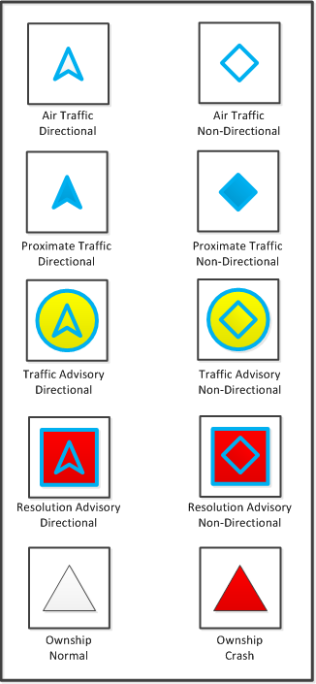
\includegraphics[scale=0.40]{TrafficIcons.png} \\

\subsection{Intruder Identification Priority}
\begin{enumerate}
\item ADS-B Tail Number
\item TCAS Intruder ID
\item Radar Intruder ID
\end{enumerate}

\section{Issues List}
No issues have been identified.

\end{document}